The result section will usually be tabulated or graphed, and each table or figure should be described, noting any interesting features – whether expected or unexpected, and in particular, inferences should relate to the original aims and objectives of the research outlined in the introduction. Results should be discussed and analysed, not simply presented blandly. Comparisons should also be drawn with the results or similar existing studies if relevant – do your results confirm or contradict those of previous research? Each table or figure should be mentioned explicitly in the text. Do not include in the project any tables or figures which are not discussed in the text. It is also worth trying to present the results in as interesting and varied way as possible – for example, including figures and charts as well as just tables.


\chapter{Results}
The result section is structured in two parts. Firstly, we highlight the empirical relationship between idiosyncratic volatility of individual stocks and the resulting forecasting performance. Secondly, we pool companies in buckets by their IV percentage, and discuss the overall forecasting performance by assessing the portfolios overall return, sign ratio and respective Sharpe ratio.

\section*{Relationship between idiosyncratic volatility of individual stocks and the resulting forecasting performance}

Our analysis is based on one-step-ahead forecasting. Once the ARMA-GARCH parameters had been estimated, we constructed the out-of-sample forecasts for each company, without updating the parameters of the model that were
obtained from the training set. The out-of-sample forecasting ability of our ARMA-GARCH forecasting model were then assessed in terms of statistical accuracy and economic criteria. 

First, the results 


Main points:

Få inn 
\begin{itemize}
    \item Graph 6.1: Vi ser en sammenehng mellom IV prosent og forecasting error. Det er altså vanskeligere å nøyaktig i størrelsesorden forutse høy IV-aksjer sin return. Dette er en pooled regression
    \item Vi bommer også mer på retning på høy IV stocks
    \item Men når vi treffer riktig retning, så er det på de store utslagene - som gjør at vi genererer positive alphaer, der alpha er definert som....
    \item Høy korrelasjon mellom IV og volatilitet - og det highlighter at vi genererer høy alpha fordi vi treffer på de store utslagene
\end{itemize}

\textbf{Table med regressjonsresultater - Alpha, beta, t-verdier, r sq.}

Table I shows the results of the goodness of forecasts for the different models and time periods and
for the corresponding forecast horizons. The main conclusions are two.

\begin{figure}[h]
    \centering
    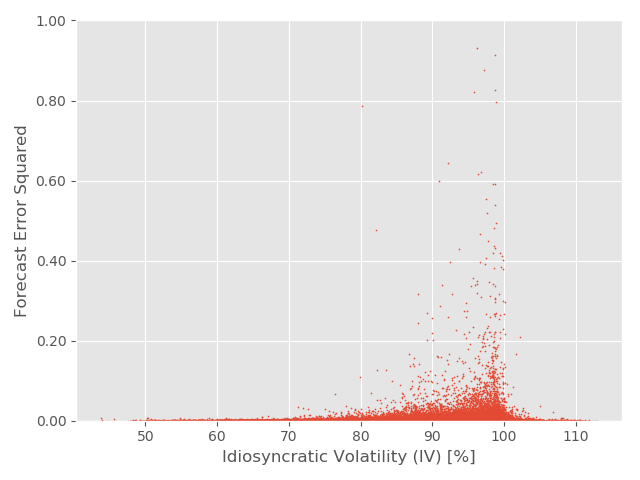
\includegraphics[scale = 1]{Plot/ScatterRegression.png}
    \caption{Regression: IV to forecasting error}
    \label{visualization}
\end{figure}

\begin{figure}[h]
    \centering
    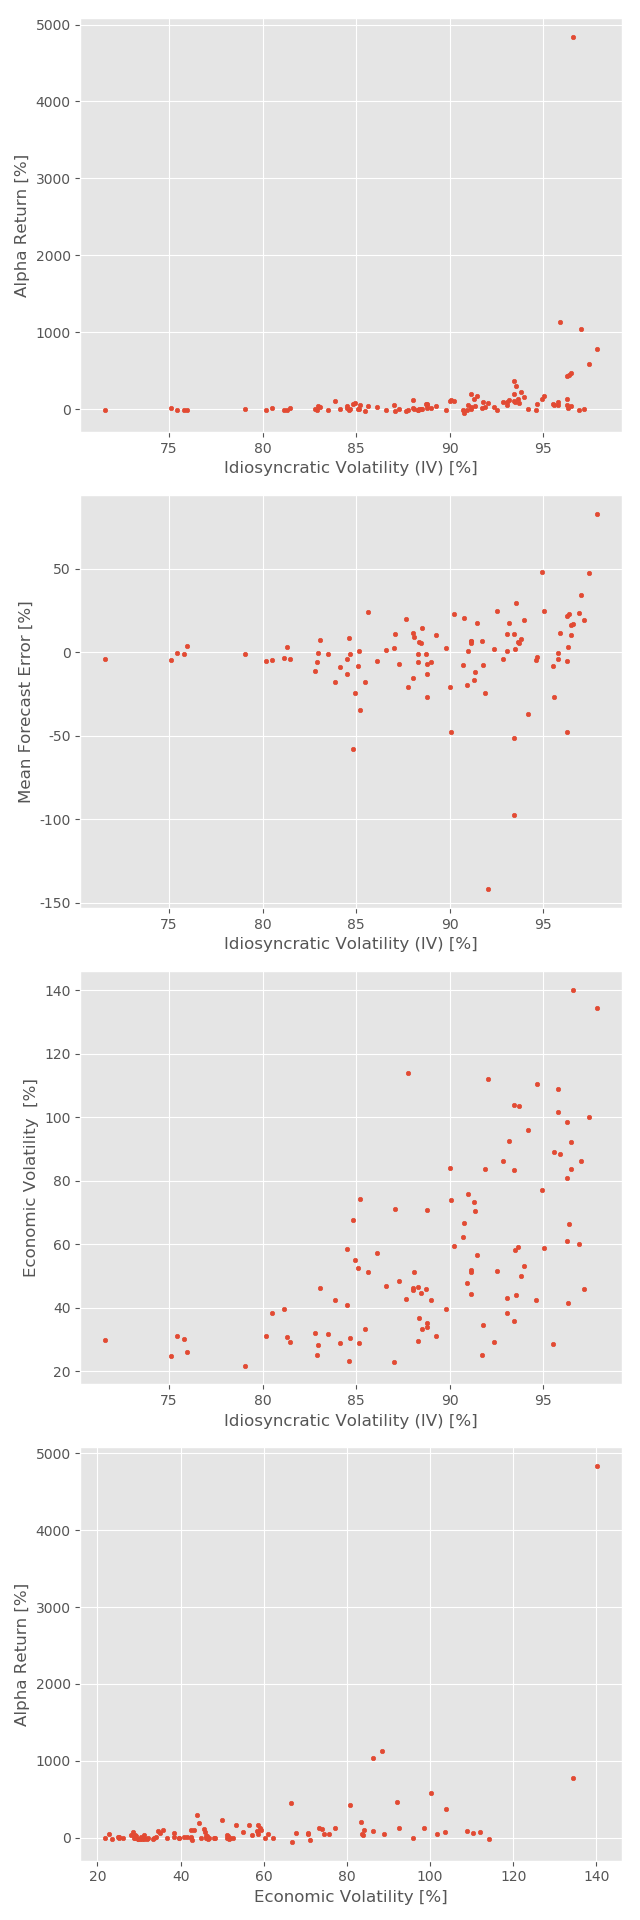
\includegraphics[height = 9 in , width = 5 in]{Plot/IndividualStockRegression.png}
    \caption{Regression: IV to forecasting error}
    \label{visualization}
\end{figure}

\section*{Forecasting performance of buckets }

\begin{itemize}
    \item Nå har vi sett på sammenhengen mellom enkeltaksjers IV og forecasting performance
    \item Nå ønsker vi å lage portføljer for å kaste lys over det samme problemet, nå med mer utjevnede forskjeller. 
    \item Når IV øker, minker sign ration, men samtidig øker alphaen, fordi vi se volatiliteten øker
    \item Kommentere sharpe ratione
\end{itemize}



\newpage
\newcolumntype{P}[1]{>{\centering\arraybackslash}p{#1}}
\begin{landscape}
\begin{longtable}{P{1.5cm}P{1.5cm}P{1.5cm}P{1.5cm}P{1.6cm}P{1.5cm}P{1.5cm}P{1.5cm}P{1.5cm}P{1.5cm}P{1.5cm}P{1.5cm}} 
\caption{Forecast Stocks}
\label{Forecast Stocks}\\
\hline
\textbf{Bucket} & \textbf{IV }$\boldsymbol{\%}$ & $\boldsymbol{r_{economic}}$ & $\boldsymbol{\sigma_{economic}}$ & \textbf{Sign Ratio} &  $\boldsymbol{r_{sign}}$ & $\boldsymbol{\sigma_{sign}}$ & $\boldsymbol{\alpha}$ & $\boldsymbol{\bar\epsilon_{forecast}}$ & $\boldsymbol{\sigma_{forecast}}$ & $\boldsymbol{S_{economic}} $ & $\boldsymbol{S_{sign}}$ \\
\hline
\endfirsthead
\multicolumn{12}{c}%
{\tablename\ \thetable\ -- \textit{Continued from previous page}} \\
\hline
\textbf{Bucket} & \textbf{IV }$\boldsymbol{\%}$ & $\boldsymbol{r_{economic}}$ & $\boldsymbol{\sigma_{economic}}$ & \textbf{Sign Ratio} &  $\boldsymbol{r_{sign}}$ & $\boldsymbol{\sigma_{sign}}$ & $\boldsymbol{\alpha}$ & $\boldsymbol{\bar\epsilon_{forecast}}$ & $\boldsymbol{\sigma_{forecast}}$ & $\boldsymbol{S_{economic}} $ & $\boldsymbol{S_{sign}}$ \\
\hline
\endhead
\hline \multicolumn{12}{r}{\textit{Continued on next page}} \\
\endfoot
\hline
\endlastfoot
\input{Input/BucketTable.txt}
\end{longtable}
\end{landscape}



